\documentclass[american,]{article}
\usepackage{lmodern}
\usepackage{amssymb,amsmath}
\usepackage{ifxetex,ifluatex}
\usepackage{fixltx2e} % provides \textsubscript
\ifnum 0\ifxetex 1\fi\ifluatex 1\fi=0 % if pdftex
  \usepackage[T1]{fontenc}
  \usepackage[utf8]{inputenc}
\else % if luatex or xelatex
  \ifxetex
    \usepackage{mathspec}
  \else
    \usepackage{fontspec}
  \fi
  \defaultfontfeatures{Ligatures=TeX,Scale=MatchLowercase}
\fi
% use upquote if available, for straight quotes in verbatim environments
\IfFileExists{upquote.sty}{\usepackage{upquote}}{}
% use microtype if available
\IfFileExists{microtype.sty}{%
\usepackage{microtype}
\UseMicrotypeSet[protrusion]{basicmath} % disable protrusion for tt fonts
}{}
\usepackage[margin=1in]{geometry}
\usepackage{hyperref}
\hypersetup{unicode=true,
            pdftitle={Will Kobe Bryant Make His Next Shot: Quadratic Discriminant Analysis and Logistic Regression using R},
            pdfauthor={Paul Adams; Reannan McDaniel; Jeff Nguyen},
            pdfborder={0 0 0},
            breaklinks=true}
\urlstyle{same}  % don't use monospace font for urls
\ifnum 0\ifxetex 1\fi\ifluatex 1\fi=0 % if pdftex
  \usepackage[shorthands=off,main=american]{babel}
\else
  \usepackage{polyglossia}
  \setmainlanguage[variant=american]{english}
\fi
\usepackage{natbib}
\bibliographystyle{apalike}
\usepackage{longtable,booktabs}
\usepackage{graphicx,grffile}
\makeatletter
\def\maxwidth{\ifdim\Gin@nat@width>\linewidth\linewidth\else\Gin@nat@width\fi}
\def\maxheight{\ifdim\Gin@nat@height>\textheight\textheight\else\Gin@nat@height\fi}
\makeatother
% Scale images if necessary, so that they will not overflow the page
% margins by default, and it is still possible to overwrite the defaults
% using explicit options in \includegraphics[width, height, ...]{}
\setkeys{Gin}{width=\maxwidth,height=\maxheight,keepaspectratio}
\IfFileExists{parskip.sty}{%
\usepackage{parskip}
}{% else
\setlength{\parindent}{0pt}
\setlength{\parskip}{6pt plus 2pt minus 1pt}
}
\setlength{\emergencystretch}{3em}  % prevent overfull lines
\providecommand{\tightlist}{%
  \setlength{\itemsep}{0pt}\setlength{\parskip}{0pt}}
\setcounter{secnumdepth}{5}
% Redefines (sub)paragraphs to behave more like sections
\ifx\paragraph\undefined\else
\let\oldparagraph\paragraph
\renewcommand{\paragraph}[1]{\oldparagraph{#1}\mbox{}}
\fi
\ifx\subparagraph\undefined\else
\let\oldsubparagraph\subparagraph
\renewcommand{\subparagraph}[1]{\oldsubparagraph{#1}\mbox{}}
\fi

%%% Use protect on footnotes to avoid problems with footnotes in titles
\let\rmarkdownfootnote\footnote%
\def\footnote{\protect\rmarkdownfootnote}

%%% Change title format to be more compact
\usepackage{titling}

% Create subtitle command for use in maketitle
\providecommand{\subtitle}[1]{
  \posttitle{
    \begin{center}\large#1\end{center}
    }
}

\setlength{\droptitle}{-2em}

  \title{Will Kobe Bryant Make His Next Shot: Quadratic Discriminant Analysis and Logistic Regression using R}
    \pretitle{\vspace{\droptitle}\centering\huge}
  \posttitle{\par}
    \author{Paul Adams \\ Reannan McDaniel \\ Jeff Nguyen}
    \preauthor{\centering\large\emph}
  \postauthor{\par}
      \predate{\centering\large\emph}
  \postdate{\par}
    \date{Master of Science in Data Science, Southern Methodist University, USA}

\usepackage{booktabs}
\usepackage{longtable}
\usepackage{array}
\usepackage{multirow}
\usepackage{wrapfig}
\usepackage{float}
\usepackage{colortbl}
\usepackage{pdflscape}
\usepackage{tabu}
\usepackage{threeparttable}
\usepackage{threeparttablex}
\usepackage[normalem]{ulem}
\usepackage{makecell}
\usepackage{xcolor}

\begin{document}
\maketitle

{
\setcounter{tocdepth}{2}
\tableofcontents
}
\hypertarget{abstract}{%
\section{\texorpdfstring{\textbf{Abstract:}}{Abstract:}}\label{abstract}}

\hypertarget{this-project-investigates-the-correlation-between-multiple-potential-explanatory-variables-and-kobe-bryants-ability-to-make-a-shot-while-playing-for-the-nba-team-los-angeles-lakers-using-data-gathered-from-1996-2015.}{%
\subsubsection{\texorpdfstring{\emph{This project investigates the correlation between multiple potential explanatory variables and Kobe Bryant's ability to make a shot while playing for the NBA team Los Angeles Lakers using data gathered from \texttt{1996}-\texttt{2015}.}}{This project investigates the correlation between multiple potential explanatory variables and Kobe Bryant's ability to make a shot while playing for the NBA team Los Angeles Lakers using data gathered from 1996-2015.}}\label{this-project-investigates-the-correlation-between-multiple-potential-explanatory-variables-and-kobe-bryants-ability-to-make-a-shot-while-playing-for-the-nba-team-los-angeles-lakers-using-data-gathered-from-1996-2015.}}

\hypertarget{introduction}{%
\section{\texorpdfstring{\textbf{Introduction}}{Introduction}}\label{introduction}}

\hypertarget{this-is-a-sample-introduction.-nothing-but-a-sample.-but-a-necessary-sample-to-preserve-space.-this-is-a-sample-introduction.-nothing-but-a-sample.-but-a-necessary-sample-to-preserve-space.-this-is-a-sample-introduction.-nothing-but-a-sample.-but-a-necessary-sample-to-preserve-space.-this-is-a-sample-introduction.-nothing-but-a-sample.-but-a-necessary-sample-to-preserve-space.-this-is-a-sample-introduction.-nothing-but-a-sample.-but-a-necessary-sample-to-preserve-space.-this-is-a-sample-introduction.-nothing-but-a-sample.-but-a-necessary-sample-to-preserve-space.-this-is-a-sample-introduction.-nothing-but-a-sample.-but-a-necessary-sample-to-preserve-space.-this-is-a-sample-introduction.-nothing-but-a-sample.-but-a-necessary-sample-to-preserve-space.-this-is-a-sample-introduction.-nothing-but-a-sample.-but-a-necessary-sample-to-preserve-space.-this-is-a-sample-introduction.-nothing-but-a-sample.-but-a-necessary-sample-to-preserve-space.-this-is-a-sample-introduction.-nothing-but-a-sample.-but-a-necessary-sample-to-preserve-space.-this-is-a-sample-introduction.-nothing-but-a-sample.-but-a-necessary-sample-to-preserve-space.-this-is-a-sample-introduction.-nothing-but-a-sample.-but-a-necessary-sample-to-preserve-space.-this-is-a-sample-introduction.-nothing-but-a-sample.-but-a-necessary-sample-to-preserve-space.-this-is-a-sample-introduction.-nothing-but-a-sample.-but-a-necessary-sample-to-preserve-space.}{%
\subsubsection{This is a sample introduction. Nothing but a sample. But a necessary sample to preserve space. This is a sample introduction. Nothing but a sample. But a necessary sample to preserve space. This is a sample introduction. Nothing but a sample. But a necessary sample to preserve space. This is a sample introduction. Nothing but a sample. But a necessary sample to preserve space. This is a sample introduction. Nothing but a sample. But a necessary sample to preserve space. This is a sample introduction. Nothing but a sample. But a necessary sample to preserve space. This is a sample introduction. Nothing but a sample. But a necessary sample to preserve space. This is a sample introduction. Nothing but a sample. But a necessary sample to preserve space. This is a sample introduction. Nothing but a sample. But a necessary sample to preserve space. This is a sample introduction. Nothing but a sample. But a necessary sample to preserve space. This is a sample introduction. Nothing but a sample. But a necessary sample to preserve space. This is a sample introduction. Nothing but a sample. But a necessary sample to preserve space. This is a sample introduction. Nothing but a sample. But a necessary sample to preserve space. This is a sample introduction. Nothing but a sample. But a necessary sample to preserve space. This is a sample introduction. Nothing but a sample. But a necessary sample to preserve space.}\label{this-is-a-sample-introduction.-nothing-but-a-sample.-but-a-necessary-sample-to-preserve-space.-this-is-a-sample-introduction.-nothing-but-a-sample.-but-a-necessary-sample-to-preserve-space.-this-is-a-sample-introduction.-nothing-but-a-sample.-but-a-necessary-sample-to-preserve-space.-this-is-a-sample-introduction.-nothing-but-a-sample.-but-a-necessary-sample-to-preserve-space.-this-is-a-sample-introduction.-nothing-but-a-sample.-but-a-necessary-sample-to-preserve-space.-this-is-a-sample-introduction.-nothing-but-a-sample.-but-a-necessary-sample-to-preserve-space.-this-is-a-sample-introduction.-nothing-but-a-sample.-but-a-necessary-sample-to-preserve-space.-this-is-a-sample-introduction.-nothing-but-a-sample.-but-a-necessary-sample-to-preserve-space.-this-is-a-sample-introduction.-nothing-but-a-sample.-but-a-necessary-sample-to-preserve-space.-this-is-a-sample-introduction.-nothing-but-a-sample.-but-a-necessary-sample-to-preserve-space.-this-is-a-sample-introduction.-nothing-but-a-sample.-but-a-necessary-sample-to-preserve-space.-this-is-a-sample-introduction.-nothing-but-a-sample.-but-a-necessary-sample-to-preserve-space.-this-is-a-sample-introduction.-nothing-but-a-sample.-but-a-necessary-sample-to-preserve-space.-this-is-a-sample-introduction.-nothing-but-a-sample.-but-a-necessary-sample-to-preserve-space.-this-is-a-sample-introduction.-nothing-but-a-sample.-but-a-necessary-sample-to-preserve-space.}}

\hypertarget{exploratory-data-analysis}{%
\section{\texorpdfstring{\textbf{Exploratory Data Analysis}}{Exploratory Data Analysis}}\label{exploratory-data-analysis}}

\hypertarget{outlier-check}{%
\subsection{\texorpdfstring{\textbf{Outlier Check}}{Outlier Check}}\label{outlier-check}}

\hypertarget{first-we-performed-a-brief-outlier-check-which-included-a-graphical-analysis-of-all-shots-taken-by-loc_x-and-loc_y.-this-graphical-analysis-indicated-a-2pt-2-point-field-goal-was-recorded-from-the-3pt-3-point-range.-upon-inspection-of-other-attributes---such-as-action-type-and-shot_zone_range---we-verified-this-shot-to-be-a-member-member-of-the-3-point-level-of-shot_type.-under-the-assumption-shots-from-beyond-the-300-inch-mark-are-more-likely-to-have-been-incorrectly-recorded-as-2-points-rather-than-an-incorrectly-recorded-location-y-we-modified-our-programming-to-transform-all-shots-where-loc_y-300-to-be-recoded-as-3pt-field-gloal.}{%
\subsubsection{\texorpdfstring{First, we performed a brief outlier check, which included a graphical analysis of all shots taken, by loc\_x and loc\_y. This graphical analysis indicated a 2PT (2-point) Field Goal was recorded from the 3PT (3-point) range. Upon inspection of other attributes - such as action type and shot\_zone\_range - we verified this shot to be a member member of the 3-point level of shot\_type. Under the assumption shots from beyond the 300 inch mark are more likely to have been incorrectly recorded as 2 points rather than an incorrectly recorded location y, we modified our programming to transform all shots where \(loc_y > 300\) to be recoded as \texttt{3PT\ Field\ Gloal}.}{First, we performed a brief outlier check, which included a graphical analysis of all shots taken, by loc\_x and loc\_y. This graphical analysis indicated a 2PT (2-point) Field Goal was recorded from the 3PT (3-point) range. Upon inspection of other attributes - such as action type and shot\_zone\_range - we verified this shot to be a member member of the 3-point level of shot\_type. Under the assumption shots from beyond the 300 inch mark are more likely to have been incorrectly recorded as 2 points rather than an incorrectly recorded location y, we modified our programming to transform all shots where loc\_y \textgreater{} 300 to be recoded as 3PT Field Gloal.}}\label{first-we-performed-a-brief-outlier-check-which-included-a-graphical-analysis-of-all-shots-taken-by-loc_x-and-loc_y.-this-graphical-analysis-indicated-a-2pt-2-point-field-goal-was-recorded-from-the-3pt-3-point-range.-upon-inspection-of-other-attributes---such-as-action-type-and-shot_zone_range---we-verified-this-shot-to-be-a-member-member-of-the-3-point-level-of-shot_type.-under-the-assumption-shots-from-beyond-the-300-inch-mark-are-more-likely-to-have-been-incorrectly-recorded-as-2-points-rather-than-an-incorrectly-recorded-location-y-we-modified-our-programming-to-transform-all-shots-where-loc_y-300-to-be-recoded-as-3pt-field-gloal.}}

\hypertarget{variable-elimination}{%
\subsection{\texorpdfstring{\textbf{Variable Elimination}}{Variable Elimination}}\label{variable-elimination}}

\hypertarget{next-we-removed-one-level-factors.-these-will-never-change-so-are-not-useful-to-the-model-including-can-cause-issues-with-model-sensitivity-since-linear-trajectories-will-be-down-weighted.-therefore-their-significance-will-be-lessened-by-the-constant-state-of-the-additional-parameters.-while-this-is-may-not-be-significant-it-is-not-condusive-to-model-quality.}{%
\subsubsection{Next, we removed one-level factors. These will never change so are not useful to the model; including can cause issues with model sensitivity since linear trajectories will be down-weighted. Therefore, their significance will be lessened by the constant state of the additional parameters. While this is may not be significant, it is not condusive to model quality.}\label{next-we-removed-one-level-factors.-these-will-never-change-so-are-not-useful-to-the-model-including-can-cause-issues-with-model-sensitivity-since-linear-trajectories-will-be-down-weighted.-therefore-their-significance-will-be-lessened-by-the-constant-state-of-the-additional-parameters.-while-this-is-may-not-be-significant-it-is-not-condusive-to-model-quality.}}

\hypertarget{addressing-multicollinearity-correlation-plot-for-visual-data-exploration}{%
\subsection{\texorpdfstring{\textbf{Addressing Multicollinearity: Correlation Plot for Visual Data Exploration}}{Addressing Multicollinearity: Correlation Plot for Visual Data Exploration}}\label{addressing-multicollinearity-correlation-plot-for-visual-data-exploration}}

\hypertarget{to-address-multicollinearity-among-quantitative-predictor-variables-a-correlation-heat-map-was-created-for-visual-inspection-of-correlation.-please-see-appendix-a-to-view-this-correlation-heat-map.}{%
\subsubsection{To address multicollinearity among quantitative predictor variables, a correlation heat map was created for visual inspection of correlation. Please see Appendix A to view this correlation heat map.}\label{to-address-multicollinearity-among-quantitative-predictor-variables-a-correlation-heat-map-was-created-for-visual-inspection-of-correlation.-please-see-appendix-a-to-view-this-correlation-heat-map.}}

\pagebreak
\cleardoublepage

\hypertarget{post-correlation-heat-map-variable-elimination}{%
\subsection{\texorpdfstring{\textbf{Post-Correlation Heat Map Variable Elimination}}{Post-Correlation Heat Map Variable Elimination}}\label{post-correlation-heat-map-variable-elimination}}

\hypertarget{following-our-correlation-heat-map-we-decided-to-eliminate-some-collinear-terms.-however-some-of-the-collinearity-is-useful-to-capture-the-instances-where-the-terms-are-unique.-for-example-combined_shot_type-factor-variable-is-collinear-with-shot_distance-quantitative-variable-but-it-also-accounts-for-the-method-kobe-may-use-to-make-a-shot.-for-example-distance-may-be-relatively-the-same-between-10-and-11-feet-but-the-factor-levels-used-to-derrive-their-short-or-far-indications-may-differ.-this-difference-could-be-whether-kobe-makes-a-potentially-more-accurate-heel-planted-shot-or-if-he-is-forced-to-lean-forward-and-take-a-riskier-shot-at-basket-the-difference-in-distance-may-only-be-one-foot-but-the-difference-in-technique-could-measure-significant-relative-to-the-odds-of-success.}{%
\subsubsection{\texorpdfstring{Following our correlation heat map, we decided to eliminate some collinear terms. However, some of the collinearity is useful to capture the instances where the terms are unique. For example, \texttt{combined\_shot\_type} (factor variable) is collinear with \texttt{shot\_distance} (quantitative variable), but it also accounts for the method Kobe may use to make a shot. For example, distance may be relatively the same between 10 and 11 feet, but the factor levels used to derrive their \texttt{short} or \texttt{far} indications may differ. This difference could be whether Kobe makes a potentially more accurate heel-planted shot or if he is forced to lean forward and take a riskier shot at basket; the difference in distance may only be one foot, but the difference in technique could measure significant relative to the odds of success.}{Following our correlation heat map, we decided to eliminate some collinear terms. However, some of the collinearity is useful to capture the instances where the terms are unique. For example, combined\_shot\_type (factor variable) is collinear with shot\_distance (quantitative variable), but it also accounts for the method Kobe may use to make a shot. For example, distance may be relatively the same between 10 and 11 feet, but the factor levels used to derrive their short or far indications may differ. This difference could be whether Kobe makes a potentially more accurate heel-planted shot or if he is forced to lean forward and take a riskier shot at basket; the difference in distance may only be one foot, but the difference in technique could measure significant relative to the odds of success.}}\label{following-our-correlation-heat-map-we-decided-to-eliminate-some-collinear-terms.-however-some-of-the-collinearity-is-useful-to-capture-the-instances-where-the-terms-are-unique.-for-example-combined_shot_type-factor-variable-is-collinear-with-shot_distance-quantitative-variable-but-it-also-accounts-for-the-method-kobe-may-use-to-make-a-shot.-for-example-distance-may-be-relatively-the-same-between-10-and-11-feet-but-the-factor-levels-used-to-derrive-their-short-or-far-indications-may-differ.-this-difference-could-be-whether-kobe-makes-a-potentially-more-accurate-heel-planted-shot-or-if-he-is-forced-to-lean-forward-and-take-a-riskier-shot-at-basket-the-difference-in-distance-may-only-be-one-foot-but-the-difference-in-technique-could-measure-significant-relative-to-the-odds-of-success.}}

\hypertarget{addressing-multicollinearity-correlation-matrix-for-numerical-analysis}{%
\subsection{\texorpdfstring{\textbf{Addressing Multicollinearity: Correlation Matrix for Numerical Analysis}}{Addressing Multicollinearity: Correlation Matrix for Numerical Analysis}}\label{addressing-multicollinearity-correlation-matrix-for-numerical-analysis}}

\hypertarget{after-deselecting-the-most-obvious-collinear-terms-through-visually-inspection-of-the-correlation-plot-a-correlation-matrix-for-analyzing-the-remaining-results.-collinear-quantitative-data-was-preliminarily-removed-following-correlation-plot-analysis-to-desaturate-the-model-to-an-extent-that-allows-more-distinction-among-significance-measures-for-terms-in-the-correlation-matrix.}{%
\subsubsection{After deselecting the most obvious collinear terms through visually inspection of the correlation plot, a correlation matrix for analyzing the remaining results. Collinear quantitative data was preliminarily removed following correlation plot analysis to desaturate the model to an extent that allows more distinction among significance measures for terms in the correlation matrix.}\label{after-deselecting-the-most-obvious-collinear-terms-through-visually-inspection-of-the-correlation-plot-a-correlation-matrix-for-analyzing-the-remaining-results.-collinear-quantitative-data-was-preliminarily-removed-following-correlation-plot-analysis-to-desaturate-the-model-to-an-extent-that-allows-more-distinction-among-significance-measures-for-terms-in-the-correlation-matrix.}}

\hypertarget{quadratic-discriminant-analysis}{%
\section{\texorpdfstring{\textbf{Quadratic Discriminant Analysis}}{Quadratic Discriminant Analysis}}\label{quadratic-discriminant-analysis}}

\hypertarget{as-requested-within-the-requirements-of-this-study-a-linear-discriminant-analysis-must-be-assessed-and-provided.-discriminant-analysis-is-an-operation-that-compares-a-categorical-response-variable-against-measures-of-quantitative-predictor-variables.-as-a-result-analysis-for-this-section-is-performed-on-the-numerical-predictors-which-include-recid-game_event_id-game_id-loc_x-loc_y-minutes_remaining-seconds_remaining-shot_distance-shot_made_flag-shot_type-game_date-shot_id-attendance-arena_temp-avgnoisedb-controlling-collinearity-by-eliminating-a-member-of-each-collinear-pair-prior-to-model-development.}{%
\subsubsection{\texorpdfstring{As requested within the requirements of this study, a Linear Discriminant Analysis must be assessed and provided. Discriminant analysis is an operation that compares a categorical response variable against measures of quantitative predictor variables. As a result, analysis for this section is performed on the numerical predictors, which include \texttt{recId}, \texttt{game\_event\_id}, \texttt{game\_id}, \texttt{loc\_x}, \texttt{loc\_y}, \texttt{minutes\_remaining}, \texttt{seconds\_remaining}, \texttt{shot\_distance}, \texttt{shot\_made\_flag}, \texttt{shot\_type}, \texttt{game\_date}, \texttt{shot\_id}, \texttt{attendance}, \texttt{arena\_temp}, \texttt{avgnoisedb}, controlling collinearity by eliminating a member of each collinear pair prior to model development.}{As requested within the requirements of this study, a Linear Discriminant Analysis must be assessed and provided. Discriminant analysis is an operation that compares a categorical response variable against measures of quantitative predictor variables. As a result, analysis for this section is performed on the numerical predictors, which include recId, game\_event\_id, game\_id, loc\_x, loc\_y, minutes\_remaining, seconds\_remaining, shot\_distance, shot\_made\_flag, shot\_type, game\_date, shot\_id, attendance, arena\_temp, avgnoisedb, controlling collinearity by eliminating a member of each collinear pair prior to model development.}}\label{as-requested-within-the-requirements-of-this-study-a-linear-discriminant-analysis-must-be-assessed-and-provided.-discriminant-analysis-is-an-operation-that-compares-a-categorical-response-variable-against-measures-of-quantitative-predictor-variables.-as-a-result-analysis-for-this-section-is-performed-on-the-numerical-predictors-which-include-recid-game_event_id-game_id-loc_x-loc_y-minutes_remaining-seconds_remaining-shot_distance-shot_made_flag-shot_type-game_date-shot_id-attendance-arena_temp-avgnoisedb-controlling-collinearity-by-eliminating-a-member-of-each-collinear-pair-prior-to-model-development.}}

\hypertarget{linear-discriminant-analysis-requires-a-linear-boundary-between-the-predictor-variables-respective-of-the-response.-if-the-boundary-between-predictors-and-response-is-not-linear-quadratic-discriminant-analysis-qda-must-be-used.-wilks-lambda-distribution-is-used-to-assess-the-nature-of-boundary-linearity-which-is-a-required-understanding-to-develop-a-well-fit-discriminant-classification-model.-however-because-of-the-large-dimensions-of-the-data-set-analyzed-in-this-study-an-approximation-of-wilks-lambda-must-be-used-rather-than-wilks-lambda-itself.-bartletts-test-is-an-approximation-of-wilks-lambda-that-can-be-used-for-models-with-large-dimensions-by-applying-a-measure-against-the-chi-square-distribution.-this-method-is-applied-herein-to-assess-linearity.}{%
\subsubsection{\texorpdfstring{\texttt{Linear\ Discriminant\ Analysis} requires a linear boundary between the predictor variables, respective of the response. If the boundary between predictors and response is not linear, \texttt{Quadratic\ Discriminant\ Analysis} (QDA) must be used. \texttt{Wilks\textquotesingle{}\ Lambda} distribution is used to assess the nature of boundary linearity, which is a required understanding to develop a well-fit discriminant classification model. However, because of the large dimensions of the data set analyzed in this study, an approximation of Wilks' Lambda must be used, rather than Wilks' Lambda itself. \texttt{Bartlett\textquotesingle{}s\ Test} is an approximation of Wilks' Lambda that can be used for models with large dimensions by applying a measure against the \texttt{Chi-Square\ distribution}. This method is applied herein to assess linearity.}{Linear Discriminant Analysis requires a linear boundary between the predictor variables, respective of the response. If the boundary between predictors and response is not linear, Quadratic Discriminant Analysis (QDA) must be used. Wilks' Lambda distribution is used to assess the nature of boundary linearity, which is a required understanding to develop a well-fit discriminant classification model. However, because of the large dimensions of the data set analyzed in this study, an approximation of Wilks' Lambda must be used, rather than Wilks' Lambda itself. Bartlett's Test is an approximation of Wilks' Lambda that can be used for models with large dimensions by applying a measure against the Chi-Square distribution. This method is applied herein to assess linearity.}}\label{linear-discriminant-analysis-requires-a-linear-boundary-between-the-predictor-variables-respective-of-the-response.-if-the-boundary-between-predictors-and-response-is-not-linear-quadratic-discriminant-analysis-qda-must-be-used.-wilks-lambda-distribution-is-used-to-assess-the-nature-of-boundary-linearity-which-is-a-required-understanding-to-develop-a-well-fit-discriminant-classification-model.-however-because-of-the-large-dimensions-of-the-data-set-analyzed-in-this-study-an-approximation-of-wilks-lambda-must-be-used-rather-than-wilks-lambda-itself.-bartletts-test-is-an-approximation-of-wilks-lambda-that-can-be-used-for-models-with-large-dimensions-by-applying-a-measure-against-the-chi-square-distribution.-this-method-is-applied-herein-to-assess-linearity.}}

\pagebreak
\clearpage

\hypertarget{bartletts-test}{%
\subsection{\texorpdfstring{\textbf{Bartlett's Test}}{Bartlett's Test}}\label{bartletts-test}}

\hypertarget{the-result-of-the-bartletts-test-returned-statistically-significant-results-indicating-the-null-hypothesis-of-linearity-must-be-rejected-in-favor-of-the-alternate-which-is-that-the-discriminant-boundary-is-non-linear.-consequently-we-proceed-with-a-model-based-on-quadratic-discriminant-analysis-to-provide-predictive-responses-from-a-discriminant-model.-however-we-proceed-with-caution-as-the-quadratic-version-of-the-discriminant-analysis-is-at-greater-risk-for-over-fitting-to-the-data-than-linear-discriminant-analysis-as-the-boundary-is-required-to-conform-more-closely-to-the-data-rather-than-to-the-mean-of-the-data.-this-was-also-taken-into-consideration-when-assessing-the-results-of-the-logistic-regression-model-development-that-occurs-afterward.-bartletts-test-of-this-data-set-yielded-a-significant-p-value-where-p-0.0001-indicating-that-the-proportion-of-distribution-beyond-the-derrived-test-statistic-is-beyond-that-which-could-be-explained-by-chance.-therefore-we-must-reject-the-null-hypothesis-that-the-boundary-for-analysis-is-linear-the-boundary-is-non-linear.-thus-an-analysis-using-quadratic-discriminant-analysis-is-applied.}{%
\subsubsection{\texorpdfstring{The result of the Bartlett's test returned statistically significant results, indicating the null hypothesis of linearity must be rejected in favor of the alternate, which is that the discriminant boundary is non-linear. Consequently, we proceed with a model based on \texttt{Quadratic\ Discriminant\ Analysis} to provide predictive responses from a discriminant model. However, we proceed with caution, as the quadratic version of the discriminant analysis is at greater risk for over-fitting to the data than Linear Discriminant Analysis as the boundary is required to conform more closely to the data rather than to the mean of the data. This was also taken into consideration when assessing the results of the Logistic Regression model development that occurs afterward. Bartlett's Test of this data set yielded a significant p-value, where p \textless{} 0.0001, indicating that the proportion of distribution beyond the derrived test statistic is beyond that which could be explained by chance. Therefore, we must reject the null hypothesis that the boundary for analysis is linear; the boundary is non-linear. Thus, an analysis using Quadratic Discriminant Analysis is applied.}{The result of the Bartlett's test returned statistically significant results, indicating the null hypothesis of linearity must be rejected in favor of the alternate, which is that the discriminant boundary is non-linear. Consequently, we proceed with a model based on Quadratic Discriminant Analysis to provide predictive responses from a discriminant model. However, we proceed with caution, as the quadratic version of the discriminant analysis is at greater risk for over-fitting to the data than Linear Discriminant Analysis as the boundary is required to conform more closely to the data rather than to the mean of the data. This was also taken into consideration when assessing the results of the Logistic Regression model development that occurs afterward. Bartlett's Test of this data set yielded a significant p-value, where p \textless{} 0.0001, indicating that the proportion of distribution beyond the derrived test statistic is beyond that which could be explained by chance. Therefore, we must reject the null hypothesis that the boundary for analysis is linear; the boundary is non-linear. Thus, an analysis using Quadratic Discriminant Analysis is applied.}}\label{the-result-of-the-bartletts-test-returned-statistically-significant-results-indicating-the-null-hypothesis-of-linearity-must-be-rejected-in-favor-of-the-alternate-which-is-that-the-discriminant-boundary-is-non-linear.-consequently-we-proceed-with-a-model-based-on-quadratic-discriminant-analysis-to-provide-predictive-responses-from-a-discriminant-model.-however-we-proceed-with-caution-as-the-quadratic-version-of-the-discriminant-analysis-is-at-greater-risk-for-over-fitting-to-the-data-than-linear-discriminant-analysis-as-the-boundary-is-required-to-conform-more-closely-to-the-data-rather-than-to-the-mean-of-the-data.-this-was-also-taken-into-consideration-when-assessing-the-results-of-the-logistic-regression-model-development-that-occurs-afterward.-bartletts-test-of-this-data-set-yielded-a-significant-p-value-where-p-0.0001-indicating-that-the-proportion-of-distribution-beyond-the-derrived-test-statistic-is-beyond-that-which-could-be-explained-by-chance.-therefore-we-must-reject-the-null-hypothesis-that-the-boundary-for-analysis-is-linear-the-boundary-is-non-linear.-thus-an-analysis-using-quadratic-discriminant-analysis-is-applied.}}

\hypertarget{following-the-removal-of-predictor-variables-after-visually-inspecting-the-correlation-heat-map-we-analyzed-a-correlation-matrix.-however-the-matrix-itself-did-not-identify-any-remaining-collinearity-at-a-threshold-of-correlation-necessitating-removal-of-like-terms.-consequently-no-further-predictor-variables-are-removed.-therefore-modeling-data-is-broken-into-a-75-training-25-testing-data-split-for-internal-cross-cross-validation.-the-objective-of-internal-cross-validation-is-to-develop-a-model-using-75-of-the-data-and-test-it-on-the-remaining-25-in-order-to-assess-model-fit-statistics.-typically-following-internal-cross-validation-external-cross-validation-is-performed.}{%
\subsubsection{Following the removal of predictor variables after visually inspecting the correlation heat map, we analyzed a correlation matrix. However, the matrix itself did not identify any remaining collinearity at a threshold of correlation necessitating removal of like-terms. Consequently, no further predictor variables are removed. Therefore, modeling data is broken into a 75\% training / 25\% testing data split for internal cross-cross validation. The objective of internal cross-validation is to develop a model using 75\% of the data and test it on the remaining 25\% in order to assess model fit statistics. Typically, following internal cross-validation, external cross-validation is performed.}\label{following-the-removal-of-predictor-variables-after-visually-inspecting-the-correlation-heat-map-we-analyzed-a-correlation-matrix.-however-the-matrix-itself-did-not-identify-any-remaining-collinearity-at-a-threshold-of-correlation-necessitating-removal-of-like-terms.-consequently-no-further-predictor-variables-are-removed.-therefore-modeling-data-is-broken-into-a-75-training-25-testing-data-split-for-internal-cross-cross-validation.-the-objective-of-internal-cross-validation-is-to-develop-a-model-using-75-of-the-data-and-test-it-on-the-remaining-25-in-order-to-assess-model-fit-statistics.-typically-following-internal-cross-validation-external-cross-validation-is-performed.}}

\hypertarget{quadratic-discriminant-analysis-internal-cross-valdiation-and-model-development}{%
\section{\texorpdfstring{\textbf{Quadratic Discriminant Analysis: Internal Cross-Valdiation and Model Development}}{Quadratic Discriminant Analysis: Internal Cross-Valdiation and Model Development}}\label{quadratic-discriminant-analysis-internal-cross-valdiation-and-model-development}}

\hypertarget{following-removal-of-significant-levels-of-multicollinearity-from-the-dataset-and-partitioning-into-a-75-training-25-testing-split-internal-cross-validation-is-performed.-the-specifics-of-this-test-involves-25-folds-of-the-data---meaning-the-75-training-data-is-divided-into-25-partitions.-the-model-is-then-trainied-on-125th-of-the-original-75-then-tested-against-the-remaining-2425ths-125ths-at-a-time.-this-test-is-repeated-5-times-with-each-repeat-involving-a-different-random-partitioning-of-the-25-specified-folds-of-the-data.-finally-the-model-developed-using-the-75-training-split-is-then-applied-to-the-25-testing-split-and-predictions-are-measured-against-the-actuals-of-that-split-to-develop-model-statistics-such-as-accuracy-misclassification-precision-sensitivity-and-specificity.}{%
\subsubsection{\texorpdfstring{Following removal of significant levels of multicollinearity from the dataset and partitioning into a 75\% training / 25\% testing split, internal cross-validation is performed. The specifics of this test involves 25 folds of the data - meaning the 75\% training data is divided into 25 partitions. The model is then trainied on 1/25th of the original 75\%, then tested against the remaining 24/25ths, 1/25ths at-a-time. This test is repeated 5 times, with each repeat involving a different random partitioning of the 25 specified \texttt{folds} of the data. Finally, the model developed using the 75\% training split is then applied to the 25\% testing split and predictions are measured against the actuals of that split to develop model statistics such as \texttt{Accuracy}, \texttt{Misclassification}, \texttt{Precision}, \texttt{Sensitivity} and \texttt{Specificity}.}{Following removal of significant levels of multicollinearity from the dataset and partitioning into a 75\% training / 25\% testing split, internal cross-validation is performed. The specifics of this test involves 25 folds of the data - meaning the 75\% training data is divided into 25 partitions. The model is then trainied on 1/25th of the original 75\%, then tested against the remaining 24/25ths, 1/25ths at-a-time. This test is repeated 5 times, with each repeat involving a different random partitioning of the 25 specified folds of the data. Finally, the model developed using the 75\% training split is then applied to the 25\% testing split and predictions are measured against the actuals of that split to develop model statistics such as Accuracy, Misclassification, Precision, Sensitivity and Specificity.}}\label{following-removal-of-significant-levels-of-multicollinearity-from-the-dataset-and-partitioning-into-a-75-training-25-testing-split-internal-cross-validation-is-performed.-the-specifics-of-this-test-involves-25-folds-of-the-data---meaning-the-75-training-data-is-divided-into-25-partitions.-the-model-is-then-trainied-on-125th-of-the-original-75-then-tested-against-the-remaining-2425ths-125ths-at-a-time.-this-test-is-repeated-5-times-with-each-repeat-involving-a-different-random-partitioning-of-the-25-specified-folds-of-the-data.-finally-the-model-developed-using-the-75-training-split-is-then-applied-to-the-25-testing-split-and-predictions-are-measured-against-the-actuals-of-that-split-to-develop-model-statistics-such-as-accuracy-misclassification-precision-sensitivity-and-specificity.}}

\hypertarget{quadratic-discriminant-analysis-external-cross-valdiation-and-model-development}{%
\section{\texorpdfstring{\textbf{Quadratic Discriminant Analysis: External Cross-Valdiation and Model Development}}{Quadratic Discriminant Analysis: External Cross-Valdiation and Model Development}}\label{quadratic-discriminant-analysis-external-cross-valdiation-and-model-development}}

\pagebreak

\hypertarget{after-building-a-model-using-internal-cross-validation-which-applied-5-repeated-internal-cross-validations-across-the-25-folds-of-training-data-a-confusion-matrix-was-constructed-and-analyzed.-next-we-applied-the-model-developed-using-the-75-training-split-to-make-predictions-against-the-entire-portion-of-data-that-includes-values-for-shot_made_flag-in-order-to-assess-how-closely-the-model-can-predict-against-the-entire-data-set-compared-to-the-actuals.-applying-the-model-to-the-entire-dataset-as-external-cross-validation-provides-the-model-an-opportunity-to-test-against-different-data-and-more-closely-simulate-a-real-life-scenario-than-internal-cross-validation.-internal-and-external-cross-validation-is-performed-for-later-logistic-regression-models-as-well.following-external-cross-validation-of-both-models-the-metrics-are-compared-to-determine-the-best-model-quadratic-discriminant-analysis-versus-logistic-regression.}{%
\subsubsection{\texorpdfstring{After building a model using internal cross-validation, which applied 5 repeated internal cross-validations across the 25 folds of training data, a confusion matrix was constructed and analyzed. Next, we applied the model developed using the 75\% training split to make predictions against the entire portion of data that includes values for \texttt{shot\_made\_flag} in order to assess how closely the model can predict against the entire data set compared to the actuals. Applying the model to the entire dataset as \texttt{external\ cross-validation} provides the model an opportunity to test against different data and more closely simulate a real-life scenario than internal cross-validation. Internal and external cross-validation is performed for later Logistic Regression models as well.Following external cross-validation of both models, the metrics are compared to determine the best model (Quadratic Discriminant Analysis versus Logistic Regression).}{After building a model using internal cross-validation, which applied 5 repeated internal cross-validations across the 25 folds of training data, a confusion matrix was constructed and analyzed. Next, we applied the model developed using the 75\% training split to make predictions against the entire portion of data that includes values for shot\_made\_flag in order to assess how closely the model can predict against the entire data set compared to the actuals. Applying the model to the entire dataset as external cross-validation provides the model an opportunity to test against different data and more closely simulate a real-life scenario than internal cross-validation. Internal and external cross-validation is performed for later Logistic Regression models as well.Following external cross-validation of both models, the metrics are compared to determine the best model (Quadratic Discriminant Analysis versus Logistic Regression).}}\label{after-building-a-model-using-internal-cross-validation-which-applied-5-repeated-internal-cross-validations-across-the-25-folds-of-training-data-a-confusion-matrix-was-constructed-and-analyzed.-next-we-applied-the-model-developed-using-the-75-training-split-to-make-predictions-against-the-entire-portion-of-data-that-includes-values-for-shot_made_flag-in-order-to-assess-how-closely-the-model-can-predict-against-the-entire-data-set-compared-to-the-actuals.-applying-the-model-to-the-entire-dataset-as-external-cross-validation-provides-the-model-an-opportunity-to-test-against-different-data-and-more-closely-simulate-a-real-life-scenario-than-internal-cross-validation.-internal-and-external-cross-validation-is-performed-for-later-logistic-regression-models-as-well.following-external-cross-validation-of-both-models-the-metrics-are-compared-to-determine-the-best-model-quadratic-discriminant-analysis-versus-logistic-regression.}}

\hypertarget{a-confusion-matrix-is-a-table-of-results-from-cross-validation.-some-key-metrics-provided-by-a-confusion-matrix-include-accuracy-precision-sensitivity-and-specificity.-accuracy-is-the-number-of-all-correct-predictions-divided-by-the-number-of-all-predictions.-precision-is-the-ratio-of-the-number-of-correctly-classified-positive-predictions-divided-by-the-number-of-all-positive-predictions.-sensitivity-also-called-recall-is-the-number-of-correctly-classified-positive-predictions-divided-by-all-positive-actuals---this-is-similiar-to-precision-except-that-sensitivity-measures-against-actual-values.-specificity-is-the-number-of-correctly-classified-negative-predictions-divided-by-all-negative-actuals.-simplistically-sensitivity-is-the-true-positive-rate-wherease-specificity-is-the-true-negative-rate.-higher-accuracy-precision-sensitivity-and-specificity-is-desireable.}{%
\subsubsection{\texorpdfstring{A confusion matrix is a table of results from cross-validation. Some key metrics provided by a confusion matrix include \texttt{Accuracy}, \texttt{Precision}, \texttt{Sensitivity} and \texttt{Specificity}. \texttt{Accuracy} is the number of all correct predictions divided by the number of all predictions. \texttt{Precision} is the ratio of the number of correctly classified positive predictions divided by the number of all positive predictions. \texttt{Sensitivity} (also called \texttt{Recall}) is the number of correctly classified positive predictions divided by all positive actuals - this is similiar to precision, except that sensitivity measures against actual values. \texttt{Specificity} is the number of correctly classified negative predictions divided by all negative actuals. Simplistically, sensitivity is the true positive rate wherease specificity is the true negative rate. Higher Accuracy, Precision, Sensitivity, and Specificity is desireable.}{A confusion matrix is a table of results from cross-validation. Some key metrics provided by a confusion matrix include Accuracy, Precision, Sensitivity and Specificity. Accuracy is the number of all correct predictions divided by the number of all predictions. Precision is the ratio of the number of correctly classified positive predictions divided by the number of all positive predictions. Sensitivity (also called Recall) is the number of correctly classified positive predictions divided by all positive actuals - this is similiar to precision, except that sensitivity measures against actual values. Specificity is the number of correctly classified negative predictions divided by all negative actuals. Simplistically, sensitivity is the true positive rate wherease specificity is the true negative rate. Higher Accuracy, Precision, Sensitivity, and Specificity is desireable.}}\label{a-confusion-matrix-is-a-table-of-results-from-cross-validation.-some-key-metrics-provided-by-a-confusion-matrix-include-accuracy-precision-sensitivity-and-specificity.-accuracy-is-the-number-of-all-correct-predictions-divided-by-the-number-of-all-predictions.-precision-is-the-ratio-of-the-number-of-correctly-classified-positive-predictions-divided-by-the-number-of-all-positive-predictions.-sensitivity-also-called-recall-is-the-number-of-correctly-classified-positive-predictions-divided-by-all-positive-actuals---this-is-similiar-to-precision-except-that-sensitivity-measures-against-actual-values.-specificity-is-the-number-of-correctly-classified-negative-predictions-divided-by-all-negative-actuals.-simplistically-sensitivity-is-the-true-positive-rate-wherease-specificity-is-the-true-negative-rate.-higher-accuracy-precision-sensitivity-and-specificity-is-desireable.}}

\hypertarget{another-important-component-for-cross-validation-is-the-misclassification-rate.-the-misclassification-rate-is-a-descriptor-of-how-often-a-model-is-wrong.-this-value-is-equal-to-the-total-number-of-false-positives-plus-the-false-negatives-divided-by-all-predictions.-a-lower-misclassification-rate-is-desireable.}{%
\subsubsection{\texorpdfstring{Another important component for cross-validation is the \texttt{Misclassification\ Rate}. The Misclassification Rate is a descriptor of how often a model is wrong. This value is equal to the total number of False Positives plus the False Negatives divided by all predictions. A lower misclassification rate is desireable.}{Another important component for cross-validation is the Misclassification Rate. The Misclassification Rate is a descriptor of how often a model is wrong. This value is equal to the total number of False Positives plus the False Negatives divided by all predictions. A lower misclassification rate is desireable.}}\label{another-important-component-for-cross-validation-is-the-misclassification-rate.-the-misclassification-rate-is-a-descriptor-of-how-often-a-model-is-wrong.-this-value-is-equal-to-the-total-number-of-false-positives-plus-the-false-negatives-divided-by-all-predictions.-a-lower-misclassification-rate-is-desireable.}}

\hypertarget{in-addition-to-the-misclassification-rate-accuracy-precision-sensitivity-specificity-and-misclassification-rate-the-logarithmic-loss-function-is-applied-to-measure-.-a-lower-logarithmic-loss-value-is-desireable-as-logarithmic-loss-increases-as-predicted-probability-diverges-from-the-actual-response-values-and-conversely-decreases-as-predicted-probability-moves-converges-toward-the-actual-response-values.}{%
\subsubsection{In addition to the misclassification rate, Accuracy, Precision, Sensitivity, Specificity and Misclassification Rate, the Logarithmic Loss function is applied to measure . A lower logarithmic loss value is desireable as logarithmic loss increases as predicted probability diverges from the actual response values and conversely decreases as predicted probability moves converges toward the actual response values.}\label{in-addition-to-the-misclassification-rate-accuracy-precision-sensitivity-specificity-and-misclassification-rate-the-logarithmic-loss-function-is-applied-to-measure-.-a-lower-logarithmic-loss-value-is-desireable-as-logarithmic-loss-increases-as-predicted-probability-diverges-from-the-actual-response-values-and-conversely-decreases-as-predicted-probability-moves-converges-toward-the-actual-response-values.}}

\hypertarget{two-final-metrics-used-in-this-analysis-are-the-area-under-the-curve-auc-and-receiver-operating-characteristic-roc-curve.-the-roc-bounds-an-area-the-area-which-the-auc-describes.-as-a-discrimination-threshold-changes-the-roc-visually-represents-the-correct-diagnostic-ability-of-a-binary-classification-model-and-is-a-plot-of-the-true-positive-against-the-false-positive-rate-at-those-varied-thresholds.-as-the-auc-describes-the-area-under-this-curve-a-higher-auc-is-more-desireable-than-a-lower-auc.-as-mentioned-these-metrics-will-be-analyzed-when-comparing-internal-to-external-cross-validation-to-ensure-consistency-as-well-as-between-the-qda-and-logistic-regression-models.}{%
\subsubsection{\texorpdfstring{Two final metrics used in this analysis are the \texttt{Area\ Under\ the\ Curve\ (AUC)} and \texttt{Receiver\ Operating\ Characteristic\ (ROC)\ curve}. The ROC bounds an area the area which the AUC describes. As a discrimination threshold changes, the ROC visually represents the correct diagnostic ability of a binary classification model and is a plot of the true positive against the false positive rate at those varied thresholds. As the AUC describes the area under this curve, a higher AUC is more desireable than a lower AUC. As mentioned, these metrics will be analyzed when comparing internal to external cross-validation to ensure consistency as well as between the QDA and Logistic Regression models.}{Two final metrics used in this analysis are the Area Under the Curve (AUC) and Receiver Operating Characteristic (ROC) curve. The ROC bounds an area the area which the AUC describes. As a discrimination threshold changes, the ROC visually represents the correct diagnostic ability of a binary classification model and is a plot of the true positive against the false positive rate at those varied thresholds. As the AUC describes the area under this curve, a higher AUC is more desireable than a lower AUC. As mentioned, these metrics will be analyzed when comparing internal to external cross-validation to ensure consistency as well as between the QDA and Logistic Regression models.}}\label{two-final-metrics-used-in-this-analysis-are-the-area-under-the-curve-auc-and-receiver-operating-characteristic-roc-curve.-the-roc-bounds-an-area-the-area-which-the-auc-describes.-as-a-discrimination-threshold-changes-the-roc-visually-represents-the-correct-diagnostic-ability-of-a-binary-classification-model-and-is-a-plot-of-the-true-positive-against-the-false-positive-rate-at-those-varied-thresholds.-as-the-auc-describes-the-area-under-this-curve-a-higher-auc-is-more-desireable-than-a-lower-auc.-as-mentioned-these-metrics-will-be-analyzed-when-comparing-internal-to-external-cross-validation-to-ensure-consistency-as-well-as-between-the-qda-and-logistic-regression-models.}}

\hypertarget{quadratic-discriminant-analysis-internal-vs.-external-cross-validation}{%
\section{\texorpdfstring{\textbf{Quadratic Discriminant Analysis: Internal vs.~External Cross-Validation}}{Quadratic Discriminant Analysis: Internal vs.~External Cross-Validation}}\label{quadratic-discriminant-analysis-internal-vs.-external-cross-validation}}

\hypertarget{using-the-two-confusion-matrix-output-tables-immediately-below-the-performance-across-internal-and-external-cross-validations-of-the-qda-model-can-be-compared.-as-indicated-in-those-figures-the-model-performed-highly-similarly-across-both-cross-validation-techniques-indicating-the-model-is-consistent-and-reasonably-fit-after-controlling-for-the-variables-selected-for-modeling.}{%
\subsubsection{Using the two confusion matrix output tables immediately below, the performance across internal and external cross-validations of the QDA model can be compared. As indicated in those figures, the model performed highly similarly across both cross-validation techniques, indicating the model is consistent and reasonably fit, after controlling for the variables selected for modeling.}\label{using-the-two-confusion-matrix-output-tables-immediately-below-the-performance-across-internal-and-external-cross-validations-of-the-qda-model-can-be-compared.-as-indicated-in-those-figures-the-model-performed-highly-similarly-across-both-cross-validation-techniques-indicating-the-model-is-consistent-and-reasonably-fit-after-controlling-for-the-variables-selected-for-modeling.}}

\pagebreak
\begin{table}

\centering
\begin{tabular}{lr}
\toprule
  & Internal CV Statistics\\
\midrule
Sensitivity & 0.51431\\
Specificity & 0.66761\\
Precision & 0.56104\\
Accuracy & 0.59826\\
Misclassification Rate & 0.40174\\
\addlinespace
Logarithmic Loss & 0.70127\\
Area Under the Curve & 0.40904\\
\bottomrule
\end{tabular}
\centering
\begin{tabular}{lr}
\toprule
  & External CV Statistics\\
\midrule
Sensitivity & 0.51187\\
Specificity & 0.66993\\
Precision & 0.55695\\
Accuracy & 0.59917\\
Misclassification Rate & 0.40083\\
\addlinespace
Logarithmic Loss & 0.70127\\
Area Under the Curve & 0.59090\\
\bottomrule
\end{tabular}
\end{table}
\newpage

\newpage

\hypertarget{appendix-a-images-and-tables}{%
\section{Appendix A: Images and Tables}\label{appendix-a-images-and-tables}}

\hypertarget{correlation-heat-map}{%
\subsubsection{Correlation Heat Map}\label{correlation-heat-map}}

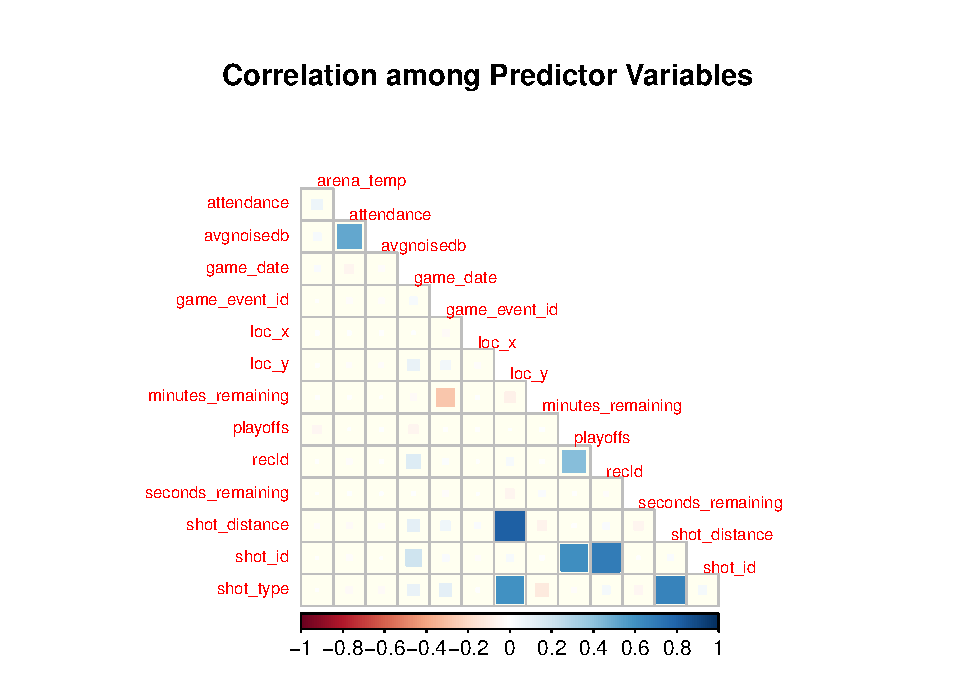
\includegraphics{Final_Project_Applied_files/figure-latex/Heatmap for Appendix-1.pdf}

\hypertarget{correlation-matrix---top-10-collinear-terms}{%
\subsubsection{Correlation Matrix - Top 10 Collinear Terms}\label{correlation-matrix---top-10-collinear-terms}}

\begin{table}[!h]
\centering
\begin{tabular}{llrl}
\toprule
Correlation Predictor Variable & Correlation Response Variable & Correlation & p-Value\\
\midrule
arena\_temp & arena\_temp & 0.51092 & p < 0.0001\\
attendance & arena\_temp & 0.51092 & p < 0.0001\\
game\_date & arena\_temp & 0.51092 & p < 0.0001\\
game\_event\_id & arena\_temp & 0.51092 & p < 0.0001\\
loc\_x & arena\_temp & 0.51092 & p < 0.0001\\
\addlinespace
loc\_y & arena\_temp & 0.51092 & p < 0.0001\\
minutes\_remaining & arena\_temp & 0.51092 & p < 0.0001\\
playoffs & arena\_temp & 0.51092 & p < 0.0001\\
recId & arena\_temp & 0.51092 & p < 0.0001\\
seconds\_remaining & arena\_temp & 0.51092 & p < 0.0001\\
\bottomrule
\end{tabular}
\end{table}

\hypertarget{bartlett-tests-wilks-lambda-approximation}{%
\subsubsection{Bartlett Test's Wilks' Lambda Approximation}\label{bartlett-tests-wilks-lambda-approximation}}

\begin{table}[t]

\caption{(\#tab:Bartletts Results for Appendix)Bartlett Test's Wilks' Lambda Approximation}
\centering
\begin{tabular}{ll}
\toprule
  & Metric Output\\
\midrule
Chi Square Statistic & 1037.24251\\
Degrees of Freedom & 14\\
Wilks' Lambda & 0.9511\\
p-Value & p < 0.0001\\
\bottomrule
\end{tabular}
\end{table}

\hypertarget{roc-curves}{%
\subsubsection{ROC Curves}\label{roc-curves}}

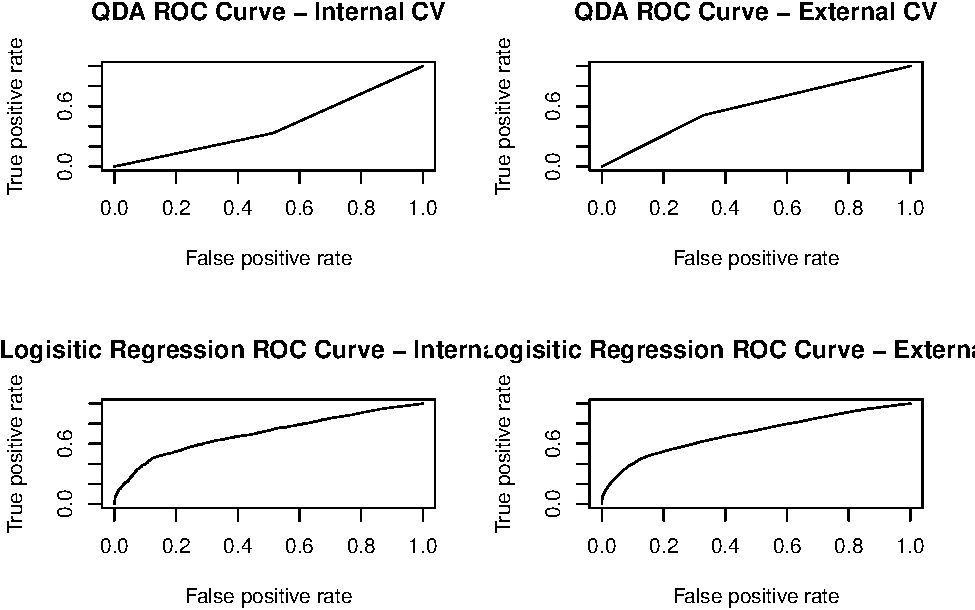
\includegraphics{Final_Project_Applied_files/figure-latex/ROC curves-1.pdf} 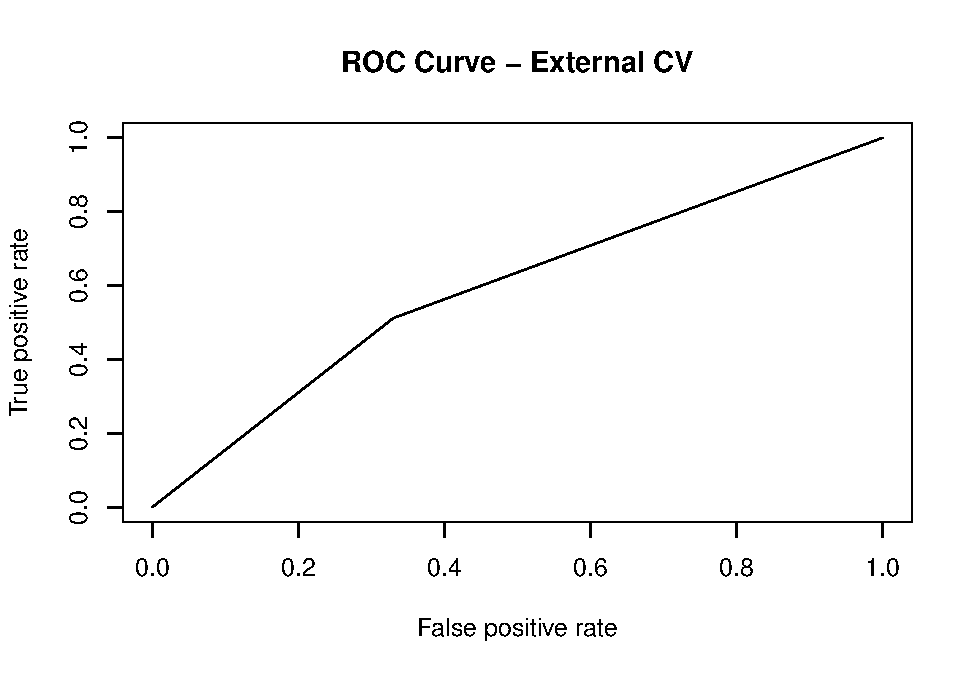
\includegraphics{Final_Project_Applied_files/figure-latex/ROC curves-2.pdf}

\bibliography{references.bib}


\end{document}
